\section{Ticket Generation}
For each HR ticket, we create a synthetic employee. For all tickets' categories, the employee has some common features: \textit{name}, \textit{first name}, \textit{last name}, \textit{nationality}, \textit{country}, \textit{email}, \textit{company}, \textit{company's email} and \textit{ticket date}.\\
All these information are created exploiting the Python library \textit{Faker}. The nationality and the company's country are selected from the extendible list \{ USA, Germany, Italy, Spain, France \}. All other information are created accordingly to the country picked. So for example if the country of birth of the employee is Italy, then the generated name will be Italian. \\
Then, once the employees are generated, the information specific to the ticket category, created starting from the open datasets as mentioned before, are concatenated to the general information of the employees. \\
For each ticket category there are distinct templates. In each template there is an initial part that contains the general information of the employee, such as name, surname, company\dots, then some prompts correlated to the category of the ticket and then the textual prompt. \\
Here's a couple of examples of templates:\\ \\
Request of time off due to health reason:
\begin{adjustwidth}{1cm}{}
From: \$\{email\} \\
To: \$\{company email\} \\
First name: \$\{first name\}\\
Last name: \$\{last name\}\\
Company: \$\{company\}\\
Date: \$\{ticket date\}\\
Ticket category: \$\{category\}\\
Ticket sub-category: \$\{sub category\} \\
Date start absence: \$\{date start absence\} \\
Reason absence: \$\{reason\} \\ 
Subject: Request for sick leave for \$\{number\_of\_days\} \\ 
\\
Dear Sir/Madame, my name is \$\{name\} and I work at \$\{company\}. I am requesting \textless \textit{generate}\textgreater. I hope \textless \textit{generate}\textgreater. \\ \\

\end{adjustwidth}
Request of refund of travel:
\begin{adjustwidth}{1cm}{}
From: \$\{email\} \\
To: \$\{company email\} \\
First name: \$\{first name\}\\
Last name: \$\{last name\}\\
Company: \$\{company\}\\
Date: \$\{ticket date\}\\
Ticket category: \$\{category\}\\
Ticket sub-category: \$\{sub category\} \\
Date Travel: \$\{date\_travel\} \\
From: \$\{airport\_from\}, \$\{from\} \\
Destination: \$\{airport\_to\}, \$\{to\} \\
\\
Hello, my name is \$\{name\}. I am writing this mail to ask a refund for the travel \textless \textit{generate}\textgreater \\ \\

\end{adjustwidth}
        
The variables are replaced with the features of the employee, whereas the \textless \textit{generate}\textgreater \space are replaced with text generated by a generative model. The part generated by the generative model are created in a recursive way. This means that the first \textless generate\textgreater \space is replaced with text generated automatically using as prompt everything that precedes it. Then the second \textless generate\textgreater \space will have as prompt the entire ticket, including the text generated previously by the model. The model is forced to generate some text, if no text is generated in an iteration, the process is repeated until the model gives a non empty output. \\

% TODO: change name of subsection
\subsection*{Architecture analysis}
To understand better how the model was behaving and why it gave certain types of outputs rather than others, we used the python library Ecco, which creates interactive visualization that show at which layers of the architecture the final token has been decided, which input tokens contribute the most for a prediction, \dots \\
In particular, we used two different methods:
\begin{itemize}
    \item Input Saliency: used to show how much did each input token contribute to producing the output token
    \item Neuron Activation Analysis: used to examine underlying patterns in neuron activations using non-negative matrix factorization
\end{itemize}
\subsubsection*{Input Saliency}
To get a better grasp of the most useful information of the prompt, and to understand how we could modify it to achieve better results, we used Gradient * input (Shrikumar et. al). This technique calculates the partial deratives off the output of the model and multiply them with the input itself. Then the inputs with the highest scores are the one that influenced the most the generation of the new tokens
\begin{equation*}
    score = x_i \bigtriangledown f(x_i)
\end{equation*}
where $f$ is the architecture output. \\
The main problem with the Gradient * input method is that only one input is considered. Integrated Gradients solve this issue, computing the average gradient while the input varies along a linear path.
\begin{equation*}
    score = (x_i - x_i')\int_{\alpha = 0}^{1} \bigtriangledown f(x' + \alpha(x - x')) \,d\alpha 
\end{equation*}
Nevertheless, we used the Gradient * input method for computational issues ( The Integrated Gradients took too much RAM of the GPUs ).\\
In the images under we underline some of the considerations we have done while defining the prompts.

\begin{figure*}[h!] 
    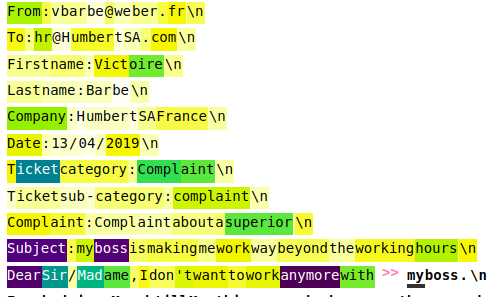
\includegraphics[width=0.6\textwidth]{images/Screenshot from 2022-11-26 17-19-27}
    \caption{Input Saliency: First token}
    \medskip
    \footnotesize
    To create the first token, the model focus on the elements that resembles the content of an email, in particular on the fact the it is indeed a 'Ticket'
    \label{fig:first_token}
\end{figure*}    

\begin{figure*}[h!] 
    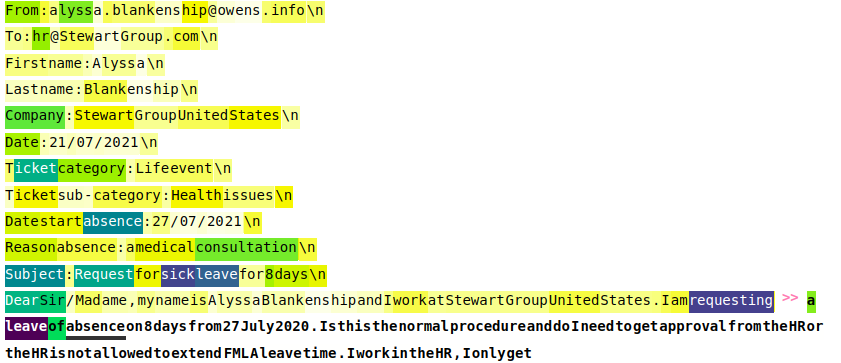
\includegraphics[width=0.8\textwidth]{images/Screenshot from 2022-11-26 18-18-28}
    \caption{Input Saliency: Subject}
    \medskip
    \footnotesize	
    Clearly stating the subject of the ticket helps the model creating tokens that are on the right topic ( In this example 'days of absence')
    \label{fig:topic}
\end{figure*}    

\begin{figure*}[h!] 
    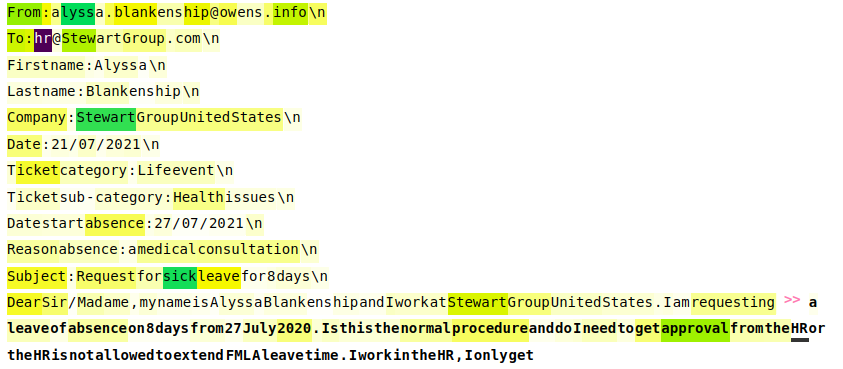
\includegraphics[width=0.85\textwidth]{images/Screenshot from 2022-11-26 18-18-40.png}
    \caption{Input Saliency: HR}
    \medskip
    \footnotesize
    Clearly stating that we are writing to hr can help the model know the context, and consecutively use a certain language, specific words\dots
    \label{fig:hr}
\end{figure*}    


\subsubsection*{Neuron Activation Analysis}
